\documentclass{beamer}
\let\vec\mathbf
\mode<presentation>
\usepackage{amsmath}
\usepackage{amssymb}
%\usepackage{advdate}
\usepackage{adjustbox}
%\usepackage{subcaption}
\usepackage{enumitem}
\usepackage{multicol}
\usepackage{mathtools}
\usepackage{listings}
\usepackage{url}
\usetheme{Boadilla}
\usecolortheme{lily}
\setbeamertemplate{footline}
{
  \leavevmode%
  \hbox{%
  \begin{beamercolorbox}[wd=\paperwidth,ht=2.25ex,dp=1ex,right]{author in head/foot}%
    \insertframenumber{} / \inserttotalframenumber\hspace*{2ex} 
  \end{beamercolorbox}}%
  \vskip0pt%
}
\setbeamertemplate{navigation symbols}{}
\providecommand{\nCr}[2]{\,^{#1}C_{#2}} % nCr
\providecommand{\nPr}[2]{\,^{#1}P_{#2}} % nPr
\providecommand{\mbf}{\mathbf}
\providecommand{\pr}[1]{\ensuremath{\Pr\left(#1\right)}}
\providecommand{\qfunc}[1]{\ensuremath{Q\left(#1\right)}}
\providecommand{\sbrak}[1]{\ensuremath{{}\left[#1\right]}}
\providecommand{\lsbrak}[1]{\ensuremath{{}\left[#1\right.}}
\providecommand{\rsbrak}[1]{\ensuremath{{}\left.#1\right]}}
\providecommand{\brak}[1]{\ensuremath{\left(#1\right)}}
\providecommand{\lbrak}[1]{\ensuremath{\left(#1\right.}}
\providecommand{\rbrak}[1]{\ensuremath{\left.#1\right)}}
\providecommand{\cbrak}[1]{\ensuremath{\left\{#1\right\}}}
\providecommand{\lcbrak}[1]{\ensuremath{\left\{#1\right.}}
\providecommand{\rcbrak}[1]{\ensuremath{\left.#1\right\}}}
\theoremstyle{remark}
\newtheorem{rem}{Remark}
\newcommand{\sgn}{\mathop{\mathrm{sgn}}}

\providecommand{\res}[1]{\Res\displaylimits_{#1}} 
\providecommand{\norm}[1]{\left\lVert#1\right\rVert}
\providecommand{\mtx}[1]{\mathbf{#1}}

\providecommand{\fourier}{\overset{\mathcal{F}}{ \rightleftharpoons}}
%\providecommand{\hilbert}{\overset{\mathcal{H}}{ \rightleftharpoons}}
\providecommand{\system}{\overset{\mathcal{H}}{ \longleftrightarrow}}
	%\newcommand{\solution}[2]{\textbf{Solution:}{#1}}
%\newcommand{\solution}{\noindent \textbf{Solution: }}align
\providecommand{\dec}[2]{\ensuremath{\overset{#1}{\underset{#2}{\gtrless}}}}
\newcommand{\myvec}[1]{\ensuremath{\begin{pmatrix}#1\end{pmatrix}}}

\title{Matrices in Geometry - 2.10.46}
\author{EE25BTECH11017 Mahesh Chollangi}
\date{Sept, 2025}

\begin{document}

\maketitle

\frame{\titlepage}
\begin{frame}{Problem Statement}
    Given vectors  $\vec{V} = 2\vec{i} + \vec{j} - \vec{k}$,  $\vec{W} = \vec{i} + 3\vec{k}$
    and $\vec{U}$ is a unit vector, find the maximum value of the scalar triple product 
    $\sbrak{\vec{U} \quad \vec{V} \quad \vec{W}}$.
\end{frame}

\section*{Solution}
\begin{frame}{Vector Representations}
    Let us express the vectors in matrix form:
    \begin{equation}
    \vec{V} = \myvec{2 \\ 1 \\ -1}, \quad \vec{W} = \myvec{1 \\ 0 \\ 3}, \quad \vec{U} = \myvec{U_x \\ U_y \\ U_z}, \quad \norm{\vec{U}} = 1.
    \label{eq:vec_def}
    \end{equation}
\end{frame}

\begin{frame}{Scalar Triple Product as a Determinant}
    The scalar triple product \(S\) is the determinant of the matrix formed by \(\vec{U}\), \(\vec{V}\), and \(\vec{W}\) as columns:
    \begin{equation}
    S = \det \begin{pmatrix}
        U_x & 2 & 1 \\
        U_y & 1 & 0 \\
        U_z & -1 & 3
    \end{pmatrix}.
    \label{eq:scalar_trip_det}
    \end{equation}
    Expanding along the first column:
    \begin{equation}
    S = U_x \det\myvec{1 & 0 \\ -1 & 3} - U_y \det\myvec{2 & 1 \\ -1 & 3} + U_z \det\myvec{2 & 1 \\ 1 & 0}.
    \label{eq:det_expansion}
    \end{equation}
\end{frame}

\begin{frame}{Determinant Evaluation}
    Calculate the minors:
    \begin{align}
    \det\myvec{1 & 0 \\ -1 & 3} &= (1)(3) - (0)(-1) = 3, \label{eq:minor1} \\
    \det\myvec{2 & 1 \\ -1 & 3} &= (2)(3) - (1)(-1) = 6 + 1 = 7, \label{eq:minor2} \\
    \det\myvec{2 & 1 \\ 1 & 0} &= (2)(0) - (1)(1) = -1. \label{eq:minor3}
    \end{align}
    Substitute back:
    \begin{equation}
    S = 3U_x - 7U_y - U_z.
    \label{eq:scalar_trip_expanded}
    \end{equation}
\end{frame}

\begin{frame}{Maximizing the Scalar Triple Product}
    Since \(\vec{U} = \myvec{U_x \\ U_y \\ U_z}\) is a unit vector,
    \begin{equation}
    U_x^2 + U_y^2 + U_z^2 = 1.
    \label{eq:unit_vec}
    \end{equation}
    Define 
    \begin{equation}
    \vec{A} = \myvec{3 \\ -7 \\ -1}.
    \label{eq:vecA_def}
    \end{equation}
    The scalar triple product reduces to the dot product
    \begin{equation}
    S = \vec{U}^\top \vec{A}.
    \label{eq:scalar_dot}
    \end{equation}

    The maximum value of \(\vec{U}^\top \vec{A}\) subject to \(\norm{\vec{U}}=1\) is 
    \begin{equation}
    \max S = \norm{\vec{A}}.
    \label{eq:max_scalar}
    \end{equation}
\end{frame}

\begin{frame}{Norm Calculation}
    Compute the norm \(\norm{\vec{A}}\):
    \begin{equation}
    \norm{\vec{A}} = \sqrt{3^2 + (-7)^2 + (-1)^2} = \sqrt{9 + 49 + 1} = \sqrt{59}.
    \label{eq:norm_calc}
    \end{equation}
\end{frame}

\begin{frame}{Final Result}
    Hence, the \textbf{maximum value} of the scalar triple product is
    \begin{equation}
    \boxed{
    \max \sbrak{\vec{U} \quad \vec{V} \quad \vec{W}} = \sqrt{59}.
    }
    \label{eq:final_answer}
    \end{equation}
\end{frame}


\begin{frame}[fragile]
\frametitle{C code}
\begin{lstlisting}

// Define vectors V and W
double V[3] = {2, 1, -1};
double W[3] = {1, 0, 3};

// Array to store cross product
double cross_V_W[3];

// Function to compute cross product
void compute_cross_product() {
    cross_V_W[0] = V[1]*W[2] - V[2]*W[1];
    cross_V_W[1] = V[2]*W[0] - V[0]*W[2];
    cross_V_W[2] = V[0]*W[1] - V[1]*W[0];
}

\end{lstlisting}
\end{frame}


\begin{frame}[fragile]
\frametitle{C code}
\begin{lstlisting}

// Functions to access cross product components
double* get_cross_product() {
    return cross_V_W;
}

\end{lstlisting}
\end{frame}

\begin{frame}[fragile]
\frametitle{Python code}
\begin{lstlisting}

import numpy as np
import matplotlib.pyplot as plt

# Define vectors V and W
V = np.array([2, 1, -1])
W = np.array([1, 0, 3])

# Compute cross product
cross_V_W = np.cross(V, W)

# Plotting the vectors and their cross product
origin = np.zeros(3)

fig = plt.figure()
ax = fig.add_subplot(111, projection='3d')


\end{lstlisting}
\end{frame}


\begin{frame}[fragile]
\frametitle{Python code}
\begin{lstlisting}

# Plot V
ax.quiver(*origin, *V, color='blue', label='V')

# Plot W
ax.quiver(*origin, *W, color='green', label='W')

# Plot cross product of V and W
ax.quiver(*origin,*cross_V_W,color='red',label='V x W')

# Setting plot limits and labels
ax.set_xlim([-3, 3])
ax.set_ylim([-3, 3])
ax.set_zlim([-3, 3])


\end{lstlisting}
\end{frame}


\begin{frame}[fragile]
\frametitle{Python code}
\begin{lstlisting}

ax.set_xlabel('X-axis')
ax.set_ylabel('Y-axis')
ax.set_zlabel('Z-axis')
ax.set_title('Vectors V, W and Cross Product V x W')

ax.legend()
plt.show()

\end{lstlisting}
\end{frame}

\begin{frame}{Plot}
    \begin{figure}[H]
    \centering
    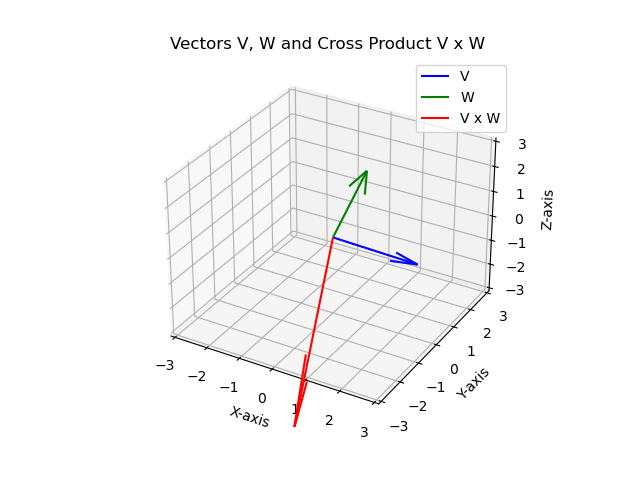
\includegraphics[width=0.8\columnwidth]{Figs/Figure_3.png}
    \caption{3D Plot}
    \label{3D Plot}
\end{figure}
\end{frame}

\end{document}
